\label{sec:dataanalysis}
Once a measurement has been made and a movie recorded the orientational dynamics are estimated. The first step is to identify the particle and approximate its position and orientation at every point. This is done using software from Johansson \cite{AntonThesis} and is explained in detail in his thesis and summarized below.

\section{Particle identification}\label{sec:particleidentification}

The first step of the data analysis is to reduce the static noise from the movie caused by dirt, scratches and other defects in the microscope and on the camera lens as can be seen in figure \ref{fig:origFrame}. As the noise is static and the actual contents of the image changes the noise is isolated by computing an average frame of all frames in a movie using equation \ref{eq:averageFrame}

An example of such an average frame can be seen in figure \ref{fig:averageFrame}. The average frame is removed from the camera frame and the result can be seen in figure \ref{fig:fixedFrame}. After this we apply a gaussian smoothing function and Canny edge detection \cite{Canny} and fill the resulting edge located closest to the previous particle location. The resulting pixels are then fit to an ellipse as described in \cite{AntonThesis, EllipseFit}, the ellipse is defined by a length $l_e$, width $w_e$ and an angle $\phi_p$ from the $x$-axis. Note that $\phi_p$ is The filled contour and the fit ellipse can be seen in figure 
\ref{fig:edgeFrame}.

\begin{figure}[H]
\centering
\begin{subfigure}[3a]{0.40\textwidth}
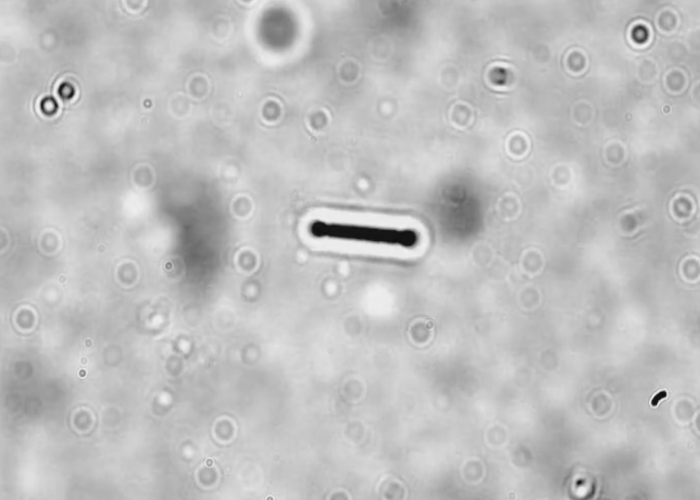
\includegraphics[width=\textwidth]{figures/method/static1.png}
\caption{A typical raw video frame.}\label{fig:origFrame}
\end{subfigure}\hspace{1em}%
\begin{subfigure}[3b]{0.40\textwidth}
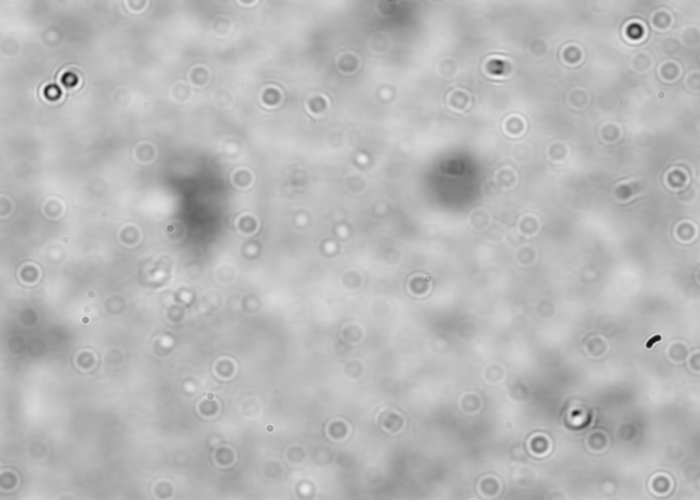
\includegraphics[width=\textwidth]{figures/method/static3.png}
\caption{The average frame $\bar{\mathbf{F}}$ from eq \ref{eq:averageFrame}.}\label{fig:averageFrame}
\end{subfigure} \\

\begin{subfigure}[3a]{0.4\textwidth}
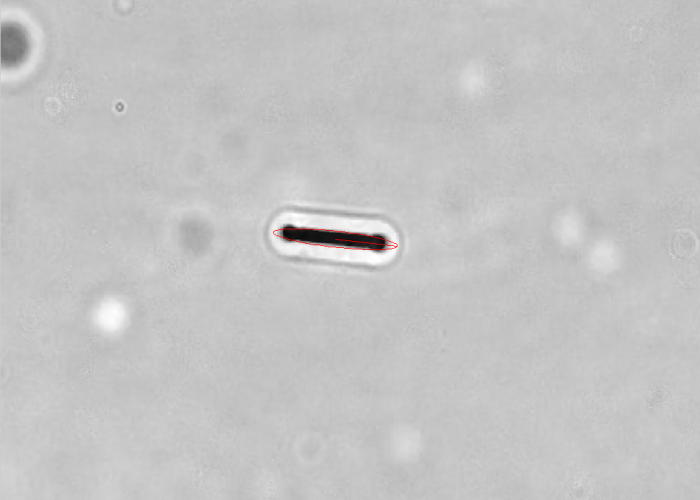
\includegraphics[width=\textwidth]{figures/method/static2.png}
\caption{The same frame after noise reduction}\label{fig:fixedFrame}
\end{subfigure}\hspace{1em}%
\begin{subfigure}[3a]{0.4\textwidth}
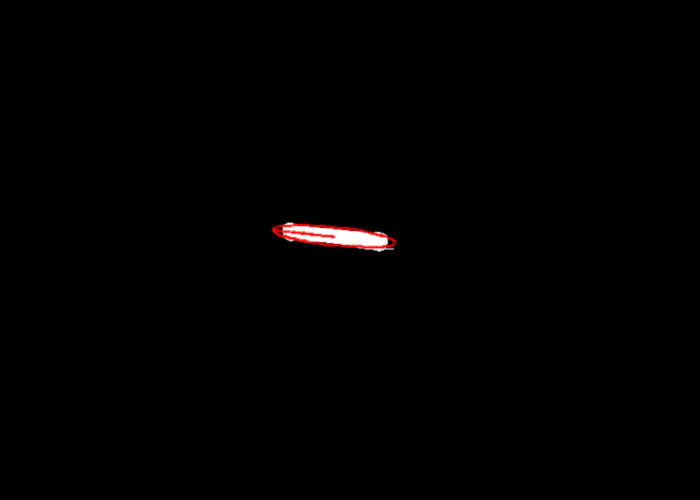
\includegraphics[width=\textwidth]{figures/method/edge.png}
\caption{After edge detection and ellipse fitting}\label{fig:edgeFrame}
\end{subfigure}

\caption{These pictures illustrate the most important step of the image analysis from raw image to estimated particle position. First the static noise from the average frame $\bar{\mathbf{F}}$}
\label{fig:detection}
\end{figure}

\section{Estimation of orientation}

The ellipsoid given by the fitting is then our best approximation of the projection in the $x$-$z$ plane. The projection of the particle along the $x$-axis and $z$-axis are found by
\begin{align} \label{eq:project}
p_x  &= l_e \sin(\phi_p) \\
p_z  &= l_e \cos(\phi_p) 
\end{align}

Here $p_x$ and $p_z$ are the $x$-axis and $z$-axis projection respectively.

To find the unit vector $\mathbf{n}$ we need to know the length of the particle. It was shown by Leal \cite{Leal} that the particle always spends a majority of its time aligned with the flow, ie aligned with the camera plane. This means that by finding the ellipse length $l_e$ every frame and finding the mode of the distribution we will find a good estimate of $L$. We find the orientation vector $\mathbf{n}$ from Section \ref{sec:jeffery} by normalizing the projections

\begin{subequations}\label{eq:normalize}
\begin{align}
n_x 	&= \frac{p_x}{L}, \\
n_z 	&= \frac{p_z}{L}, \\
n_y		&= \sqrt{1 - n_x^2 - n_z^2}.
\end{align}
\end{subequations}

This allows us to make comparisons between theory and measurement. Until this point the data analysis is the same as that in Johansson \cite{AntonThesis}.

\section{Width compensation}\label{sec:width_compensation}
We have assumed that the particle is a \emph{thin} rod so that the projection $\mathbf{p}$ onto the $x$ and $z$-axes give us an accurate estimate of $\mathbf{n}$. However, when we consider that our particle is 'thick' with length $l_e$ as well as width $w_e$ the actual unit vector we will be using in the above algorithms is $\mathbf{n}'$. The width of the particle will appear as an ellipse even when the particle is aligned completely with the $y$-axis. Looking at the points when $\phi = 0$, which are the points plotted on the surfaces of section and thus of the most 	interest, we find

\begin{equation}\label{eq:widthcomp}
\mathbf{n}' = \frac{p_z'}{L} = \frac{p_z\cos(\theta)  + D\sin(\theta)}{L} 
\end{equation}

which is illustrated in figure \ref{fig:lengtherror} for 4 different values of $\theta$. 

In order to compensate for the width of the particle we modify our projection equation \ref{eq:project} to

\begin{align}\label{eq:widthCompensation}
p_x  &= (l_e - w_e)\cdot \sin(\phi_p) \\
p_z  &= (l_e - w_e)\cdot \cos(\phi_p) 
\end{align}


This reduces the particles estimated length by $w_e$
\begin{figure}[H]
\centering
\includegraphics[width=0.6\textwidth]{figures/method/LengthError2.pdf}
\caption{Shows the incorrect projection vector $\mathbf{p}'$ we obtain from incorrectly assuming the particle is 'thin' in eq. \ref{eq:project}. The correct projection vector is highlighted in red. Shows four different $\theta$ angles at $\phi=0$.}\label{fig:lengtherror}
\end{figure} 

